\documentclass[12pt]{report}

% Essential packages for thesis
\usepackage{amssymb,amsmath,geometry,amsthm,graphicx,gensymb}
\usepackage{mathpazo}
\usepackage{float}
\usepackage{csquotes}
\usepackage[T1]{fontenc}
\usepackage{booktabs}
\usepackage{siunitx}
\usepackage{textgreek}
\usepackage{hyperref}
\usepackage{enumitem}
\usepackage[utf8]{inputenc}
\usepackage[backend=biber, style=authoryear, sorting=nyt]{biblatex}
\usepackage[dvipsnames]{xcolor}

% Package configurations
\sisetup{per-mode=symbol,detect-all}

% Bibliography
\addbibresource{reference.bib}

% Page setup
\geometry{
    paper=a4paper,
    top=2.5cm, 
    bottom=2.5cm, 
    left=2.25cm, 
    right=2.25cm, 
    headheight=14pt,
    footskip=1.00cm, 
    headsep=1.2cm, 
}

% Hyperref setup
\hypersetup{
    colorlinks=true,
    linkcolor=blue,
    citecolor=blue,
    filecolor=blue,      
    urlcolor=blue,
}

% Theorem environments
\newtheorem{thm}{Theorem}[section]
\newtheorem{cor}[thm]{Corollary}
\newtheorem{defn}[thm]{Definition}
\newtheorem{lemma}[thm]{Lemma}
\newtheorem{rmk}[thm]{Remark}
\newtheorem{eg}[thm]{Example}
\newtheorem{prop}[thm]{Proposition}
\newtheorem{qn}{Question}[chapter]
\newtheorem{prm}{Problem}[chapter]

% Mathematical commands
\newcommand{\R}{\mathbb{R}}
\newcommand{\Rd}{\R^d}
\newcommand{\C}{\mathbb{C}}
\newcommand{\Z}{\mathbb{Z}}
\newcommand{\Zd}{\mathbb{Z}^{d}}
\newcommand{\N}{\mathbb{N}}
\newcommand{\E}{\mathbb{E}}

% Operator commands
\newcommand{\norm}[1]{\|#1\|}
\newcommand{\inorm}[1]{\|#1\|_\infty}
\newcommand{\gnorm}[1]{\|#1\|_1}

% Proof environment - using standard amsthm

\begin{document}

% Title page
\pagenumbering{roman}
\thispagestyle{empty}
\begin{center}
    \vspace*{1cm}
    {\textbf{\LARGE [Your Thesis Title Here]}}\\
    
    \vspace*{1cm}
    {\large A thesis submitted in partial fulfillment of\\
    the requirements for the degree of}\\
    
    \vspace*{0.5cm}
    {\large [Your Degree]}\\
    
    \vspace*{0.5cm}
    {\large by}\\
    
    \vspace*{0.5cm}
    {\textbf{\Large [Your Full Name]}}\\
    \vspace*{0.25cm}
    {\large ([Your Student ID])}\\
    
    \vspace*{1cm}
    {\large Under the guidance of}\\
    \vspace*{0.25cm}
    {\textbf{\Large [Your Supervisor's Name]}}\\
    
    \vspace*{1.75cm}
    
    \includegraphics[width=0.3\textwidth]{logo.png}
    
    \vspace*{0.75cm}
    {\textbf{\large [Your Department Name]}}\\ \vspace*{0.2cm}
    {\textbf{\large [Your University Name]}}\\ \vspace*{0.2cm}
    {\large [Month, Year]}
    
\end{center}

% Abstract
\newpage
\chapter*{Abstract}
\addcontentsline{toc}{chapter}{Abstract}

[Your abstract goes here. This should be a concise summary of your research, typically 200-300 words. Include the main objectives, methodology, key findings, and conclusions of your work.]

% Table of contents
\newpage
\tableofcontents
\newpage

% Main content
\setcounter{page}{1}
\pagenumbering{arabic}

% Include chapters
\chapter{Introduction}

\section{Background and Motivation}
[Your background and motivation section goes here. This should introduce the general area of your research and explain why your work is important. Typically 2-3 paragraphs.] Recent studies by \textcite{chen2022emerging} have highlighted the importance of this research area.

Lorem ipsum dolor sit amet, consectetur adipiscing elit. Sed do eiusmod tempor incididunt ut labore et dolore magna aliqua. Ut enim ad minim veniam, quis nostrud exercitation ullamco laboris nisi ut aliquip ex ea commodo consequat. The work of \textcite{nguyen2020methodological} provides a solid foundation for the approach taken in this research.

\section{Research Objectives}
The main objectives of this research are:
\begin{enumerate}
\item First objective: Describe what you aim to achieve
\item Second objective: Another key goal of your research  
\item Third objective: Additional research aim if applicable
\end{enumerate}

\section{Research Questions}
This study addresses the following research questions:
\begin{enumerate}
\item Research Question 1: What specific question are you investigating?
\item Research Question 2: Another question your research addresses
\end{enumerate}

\section{Methodology Overview}
[Brief overview of your research methodology. This should be 1-2 paragraphs describing your general approach.]

\section{Example Figures}
This section demonstrates how to include figures in your thesis. Figure \ref{fig:research_overview} shows a general overview of the research process, while Figure \ref{fig:methodology} illustrates the methodology framework.

\begin{figure}[h!tbp]
\centering
\includegraphics[width=0.7\textwidth]{chapters/1/figures/fig_1.png}
\caption{Research overview and key components. This figure demonstrates how to include and reference figures in your thesis.}
\label{fig:research_overview}
\end{figure}

\begin{figure}[h!tbp]
\centering
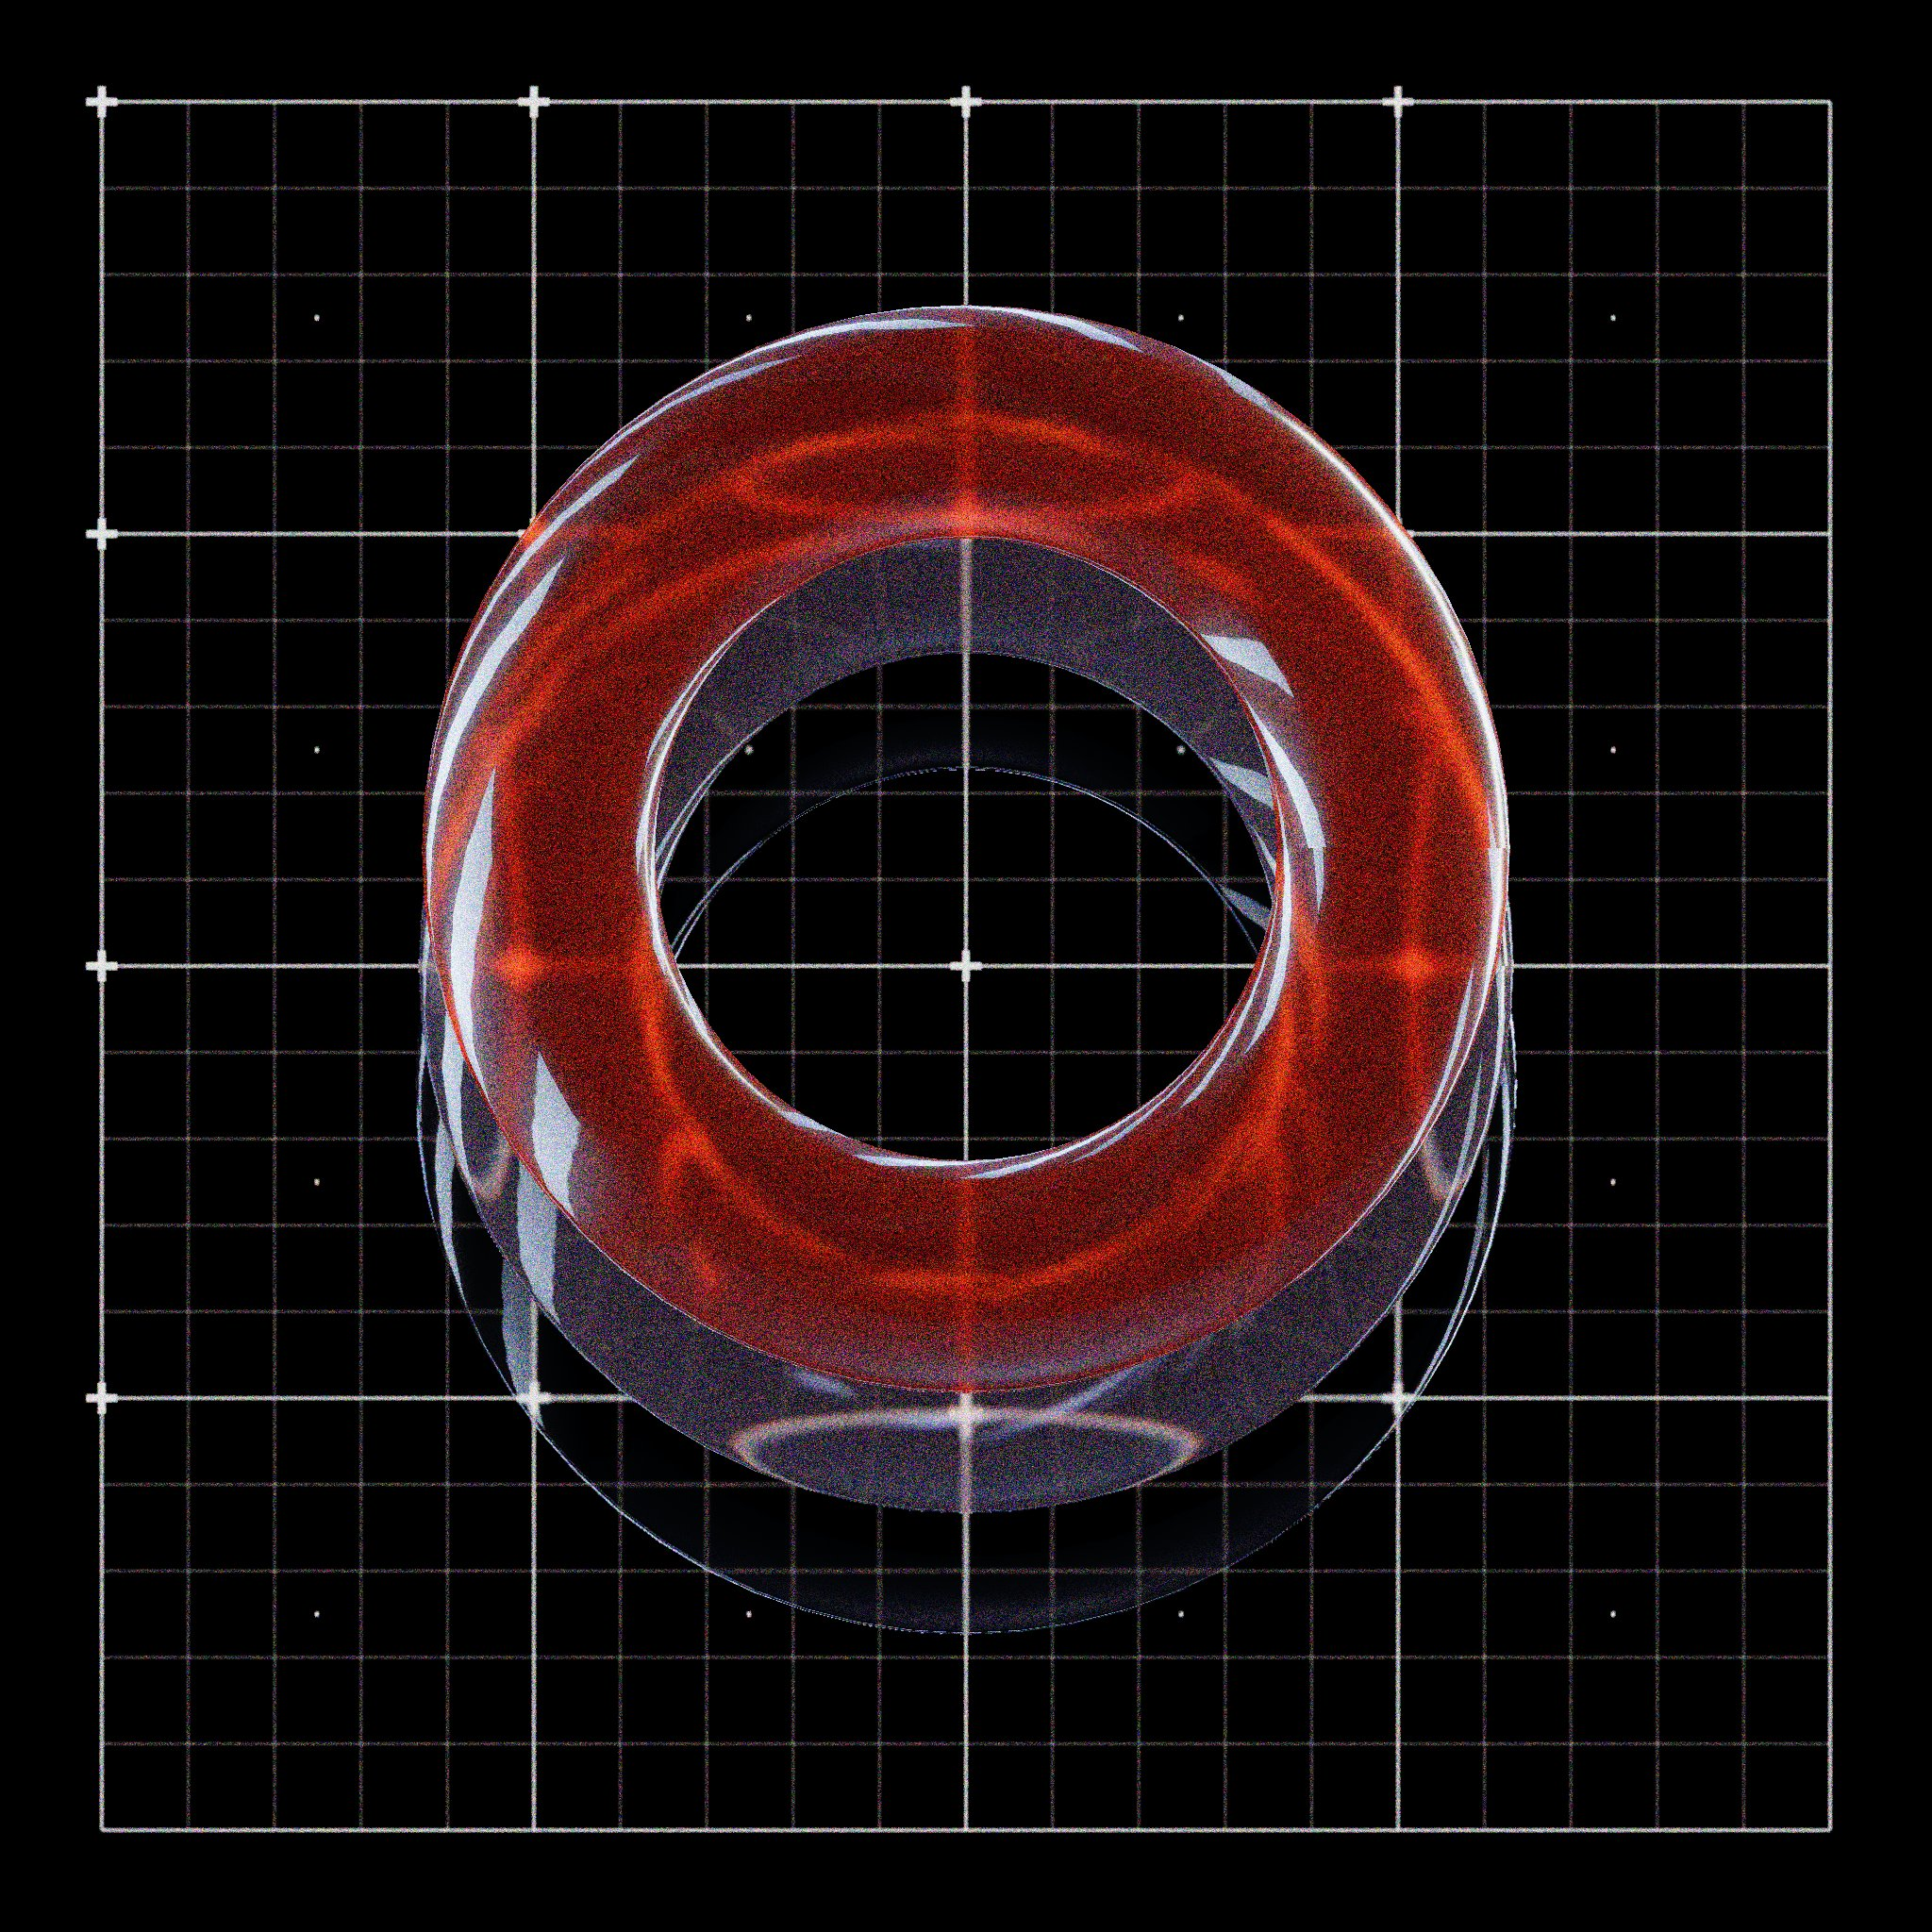
\includegraphics[width=0.7\textwidth]{chapters/1/figures/fig_2.png}
\caption{Methodology framework and approach. This shows the systematic approach to conducting research.}
\label{fig:methodology}
\end{figure}

\section{Thesis Structure}
This thesis is organized as follows:
\begin{itemize}
\item Chapter 1: Introduction - Provides background, objectives, and methodology
\item Chapter 2: Literature Review - Reviews relevant previous work and establishes context
\item Additional chapters as needed for your specific research
\end{itemize}

\section{Expected Contributions}
[Describe the expected contributions of your research to the field. What new knowledge or insights will your work provide?]

\chapter{Literature Review}

\section{Introduction to the Field}
[This section should provide an overview of the research field and establish the context for your work. Include key concepts and definitions.]

\section{Historical Development}
The field of [your research area] has evolved significantly over the past several decades. Early work by \textcite{troitskii1969electromechanical} established the fundamental principles that continue to influence current research directions. Subsequent studies by \textcite{conrad2000electroplasticity} expanded our understanding of the underlying mechanisms.

\section{Current State of Knowledge}
Recent advances in [your field] have been driven by several key developments:

\subsection{Theoretical Foundations}
The theoretical framework for understanding [your topic] was established through the work of \textcite{kim2020elucidating}, who provided a comprehensive model that explains the fundamental mechanisms involved.

\subsection{Experimental Methods}
Experimental approaches have evolved significantly, with \textcite{xu2021enhanced} introducing novel techniques that have improved our ability to measure and characterize the phenomena under investigation.

\section{Key Research Areas}
Several important areas of research have emerged in recent years:

\subsection{Area 1: [Specific Research Area]}
[Description of the first research area with relevant citations and examples.]

\subsection{Area 2: [Another Research Area]}
[Description of the second research area with relevant citations and examples.]

\section{Research Gaps and Opportunities}
Despite significant progress, several important gaps remain in our understanding:

\begin{enumerate}
\item [Gap 1: Describe what is not yet understood or investigated]
\item [Gap 2: Another area that needs further research]
\item [Gap 3: Additional research opportunities]
\end{enumerate}

\section{Example Figures}
This section demonstrates how to include figures in your literature review. Figure \ref{fig:literature_overview} provides an overview of the research landscape, while Figure \ref{fig:research_trends} shows current trends in the field.

\begin{figure}[h!tbp]
\centering
\includegraphics[width=0.7\textwidth]{chapters/2/figures/fig_1.png}
\caption{Literature overview and research landscape. This figure demonstrates how to include and reference figures in your literature review chapter.}
\label{fig:literature_overview}
\end{figure}

\begin{figure}[h!tbp]
\centering

\includegraphics[width=0.7\textwidth]{chapters/2/figures/fig_2.png}
\caption{Current research trends and developments. This shows the evolution of research in the field over time.}
\label{fig:research_trends}
\end{figure}

\section{Summary}
[Provide a summary of the key points from the literature review and how they relate to your research objectives. This should be 1-2 paragraphs.]

% Bibliography
\printbibliography[title=References]

\end{document}
